\documentclass[progress]{cmpreport}
\graphicspath{ {./images/} }

\title{GPU Accelerated Method for Constructing and Rendering Trees 
        \\ - \\ 
        Progress Report}
\author{Thomas Mcloughlin}
\date{3/12/2020}
\registration{100203952}
\ccode{CMP - 6013Y}
\supervisor{Dr. Stephen Laycock}

\begin{document}
\maketitle

\section{Description of the Project}
This section will outline the aims and motivation of the project, describing why this system 
would be useful in a 3D graphics environment application.

\subsection{Aims}
The aim of this project is to produce an OpenGL module for constructing and rendering trees 
that can be placed in a 3D environment. These trees should be randomly generated to allow 
for multiple trees to be rendered and not have them look the same. They should use a suitable 
algorithm to produce this randomness that will control the structure of branches and leaf 
placement on those branches.

\subsection{Motivation}
The motivation for producing this system is to reduce the effort that needs to be dedicated to 
creating a realistic looking 3D environment. Simulating nature can be difficult and that is 
shown in the construction of trees and other foliage. Having a designer create each tree model 
from scratch while trying to make each model look realistic and varied would be a huge 
undertaking and take a long time. Whereas using this system would allow for quick and easy 
construction and placement of trees in an environment, with user input allowing for certain 
aspects of the generated trees to be tweaked to the required specifications.

\section{Description and Understanding of Issues and Problems}
In this section the various issues and problems that have arisen during the design stage of the 
project will be listed and explained.

\subsection{Branch Structure}
The choice of what method to use for branch structure when approaching this project is the 
issue which will have the largest affect on the result. Different algorithms are likely to 
produce different results in the final branch structure so care was put in to understand the 
various methods and choose one that would be most suitable with a balance between attaining a 
realistic looking result and ease of implementation.

The choices were separated between methods described in various papers found as part of the 
Literature Review and after much consideration the decision was made to use L-systems, 
described by \cite{prusinkiewicz1996systems}, to create the branch structure in the trees. 
This would be done by creating preset constructed parts to act as our variables, using a chosen 
point in the environment as an axiom and providing the rules to construct the tree geometry. 
Some variation at each level needs to be applied to give a sense of natural growth, this would 
include a variation in branching angle each time a branch splits off from the previous branch. 
The user control can be presented through the rules of the L-system, by changing these rules 
the user could affect how the tree is constructed.

\subsection{Leaf Placement}
The problem with leaf placement is having the system decide where will be appropriate to place 
leaves to make the tree realistic looking. \cite{prusinkiewicz1996systems} combine leaf 
placement with the construction of the branches, where some variables in the chosen L-system 
include adding leaves to the constructed branch or having a terminating branch end in a leaf. 
This is decidedly too basic for use with a more detailed 3D application and so this idea will 
be combined with a method presented by \cite{weber1995rendering} where leaf placement can be 
decided based on the level of a branch. The level being the number of parental branches that 
the current branch has meaning the more parents the branch has usually means that the branch 
is further from the trunk and more likely to be a terminating branch. Leaf placement will be 
done only on branches of a certain level and above to give the trees the proper dispersion of 
leaves across outwards reaching branches.

The issue of how specifically to add leaves to the chosen branches requires another method. 
\cite{weber1995rendering} do describe their method for leaf placement somewhat but only 
give a formula for deciding the number of leaves to be placed and not specifically how they 
are placed. For this a method of random placement needs to be inferred and the chosen method 
involves these steps: decide the number of leaves needed for a chosen branch, choose varying 
points along the branch where the leaves will be placed, render the leaves, orient the leaves 
semi-randomly while taking into account the position of the tree.

\section{Design and Planning}
As a simulation project this design plan will give a design of the chosen simulation model 
supported by example pseudo code and diagrams.\\

The chosen simulation model for this project is the use of L-systems which has been loosely 
explained but will be described in more detail here.

A Lindenmayer system (L-system) is a system of ordering an alphabet of symbols to make 
strings. The symbols are formed into the string using production rules that expand each 
symbol into some larger string of symbols. The expansion starts from an initial axiom string 
which is some chosen collection of symbols, changing the axiom string is a way to alter the 
resulting string without changing any of the symbols or rules involved in the system. The 
number of times you apply the rules to the string (number of recursions) will also give you 
different strings, and a certain recursion depth may be chosen to give a desired affect.\\

\cite{prusinkiewicz1996systems} outlined multiple examples of using L-systems and below is 
a simplified explanantion of one of them and how it could be modified to correspond to this 
project.

For the production of trees with some user input required we would want to use parametric 
L-systems. The example explained below is that of a deterministic L-system (D0L-system) which 
would produce the same result every time it was ran. This is not what we want for the context 
of randomly generating trees so this method would likely be altered to become semi-deterministic 
with certain randomness in generation being added into the construction process. 

Considering the recognisable snowflake fractal we can define the multiple recursions of its 
formation using a D0L-system with this Axiom and the given Production: \\

\textbf{Axiom} $\omega$: $F(1) - (120)F(1) - (120)F(1)$ \\
\indent \textbf{Production} $p_1$: $F(s) \rightarrow F(s/3) + (60)F(s/3) - (120)F(s/3) + (60)F(s/3)$ \\

The axiom draws an equilateral triangle with edges of unit length. Productiuon $p_1$ replaces 
each line segment with a polygonal shape where the line segment has been given a convex 
triangular shape. The Production $p_1$ can be visualised as so:

\begin{figure}[h]
        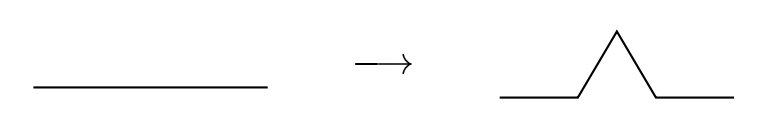
\includegraphics[scale=0.4]{production_p1}
        \centering
\end{figure}

\noindent Below are the axiom and first 3 recursions of this D0L-system:

\begin{figure}[h]
        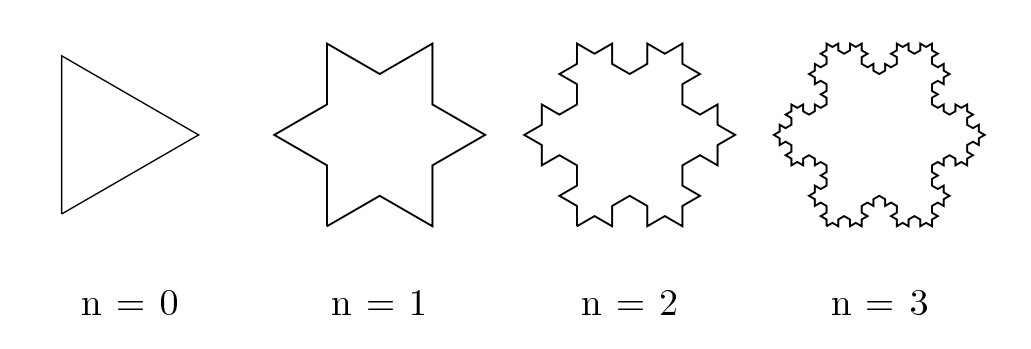
\includegraphics[scale=0.5]{triangle_snowflake_lsystem}
        \centering
\end{figure}

This basic example provides the foundation to elaborate on the planned design for the tree 
construction of this project. A semi-deterministic D0L-system will be produced that will 
allow for the generation of a general branching structure. This would be done by assigning 
3D line drawing to the symbols in our L-system that would be formed into a string. This could 
be done by building from a root point and expanding the tree branches upwards, or by starting 
with a central trunk and separating it into branches in a similar way to how the triangular 
snowflake L-system works.

The chosen symbols would represent differing thicknesses of branches as the tree expands from 
the central trunk and some symbols would include the requirement for leafs to be placed, at 
which point the chosen leaf placement method would be used to complete the branch. 

Once an acceptable default for the D0L-system has been achieved, the system can be parameterised 
to allow for user alterations of the tree generation which could include facets such as average 
branch length, number of branch splits, leaf density, tree height and width etc.

To add some random variance to the appearance of the generated trees there can be some semi 
controlled symbols that will only slightly alter the trees overall appearance. This could 
include a variation in branching angle to prevent each branch from being perfectly angled 
from it's parent. This symbol could also be parameterised to allow user control by letting 
there be a choice over what range this angle deviates.

The issue of adding thickness to the tree branches can also be combined with the L-system 
implementation. Below are some examples from another parametric L-system explained by 
\cite{prusinkiewicz1996systems} 

\begin{figure}[h]
        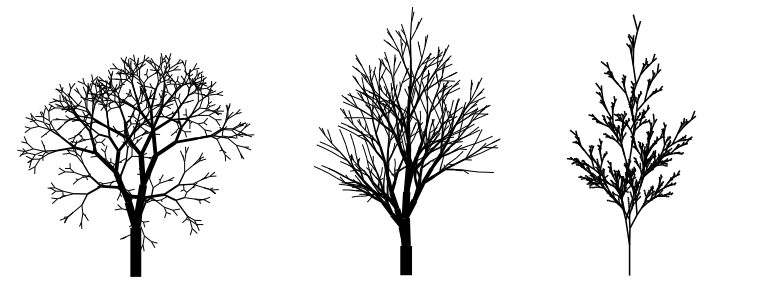
\includegraphics[scale=0.7]{tree_examples}
        \centering
\end{figure}

These trees are generated using another D0L-system that includes a parameter to increase the 
width of branch segments over each recursion which can be seen most apparently in the two 
trees on the left with their wider trunks and much thinner terminating branches. This same 
method could be applied to this project by using cylinders for each branch segment instead of 
line drawing. This would also allow for easier application of texturing to each branch as they 
will all be formed using the same shape.

\clearpage
\bibliography{bibfile}
\end{document}